\documentclass[a4paper, 11pt]{article}
\usepackage[english]{babel}
\usepackage{appendix}
\input{"/media/alessandro/OS/Users/ale57/Documents/1. universita'/ANNO IV (2019-2020)/second semester/header.tex"}

\begin{document}

\title{NNDL Homework 3: \\ Deep Reinforcement Learning}
\author{Alessandro Lovo}
\maketitle

\section{Introduction}
  This homework will deal with Reinforcement learning using \emph{OpenAI}'s \emph{gym} environments. In particular we will start with the simple \emph{CartPole}, where the goal for the agent is to balance a pole on a cart, first providing the agent with high level knowledge of the environment, then giving it just the screen pixels. Then another gym environment will be tested. In every case the goal is to consistently beat the games with as few training episodes as possible.

  \subsection{General framework}
    The interaction between the environment and the agent and learning of the latter rely on the following framework of python classes and functions:
    \begin{itemize}
      \item \textbf{Policy net}: different architectures for deep neural networks taking as input the state of the environment and providing as output the Q-values for each possible actions.
      \item \textbf{Policy}: function for choosing which action to take given the Q-values and a generic parameter $\beta$. The possible policies are:
      \emph{random} (choose action randomly, ignoring the Q-values), \emph{greedy} (choose the action with the highest Q-value), \emph{$\epsilon$-greedy} (with probability $\epsilon$ choose a non optimal action, otherwise the greedy one; here $\beta$ is $\epsilon$), \emph{softmax} (here $\beta$ is the temperature parameter and the probability of choosing action $a$ is proportional to $e^{q_a/\beta}$). Both \emph{$\epsilon$-greedy} and \emph{softmax} policies reduce to the \emph{greedy} one whe $\beta = 0$.
      \item \textbf{Agent}: class for handling the interaction with the environment: it observes the state of the environment, passes it to the \emph{policy net} obtaining the Q-values, which uses, given a \emph{policy} to choose the action to take and pass back to the environment, receiving a reward and the next state.
      \item \textbf{Replay memory}: class containing a list of finite capacity with tuples [state, action, next state, reward] from which we randomly sample when training the agent. Once we reach the maximum capacity new data will overwrite the oldest ones.
      \item \textbf{Exploration profile}: class for scheduling the value of the $\beta$ parameter for the policy of the agent at every episode of training. Said value can either be predetermined, i.e. an exponential decay with the episode number, or depend on the current performance of the agent.
      \item \textbf{Evolver}: class for handling the training of the \emph{policy net} of the \emph{Agent}. It optimizes the smooth L1 loss between  $policy\_net(state, action)$ and $reward + \gamma \cdot target\_net(next\, state, best\, action)$ where $\gamma$ is the discount rate and the target net is a periodic checkpoint of the policy net. Data [state, action, next state, reward] are sampled from the \emph{replay memory} and the best action is computed using the greedy policy on the target net.
    \end{itemize}


\section{Cart-Pole}
  This environment consist of a cart able to move on a 1d rail with a pole attached, initially facing upwards. The state consists of four real numbers: cart position ($x$), cart velocity ($v$), pole angle ($\theta$), pole angular velocity ($\omega$) and the agent has two available actions: push the cart to the right or to the left. The game ends when the pole falls ($|\theta| > 12^{\circ}$) or the cart goes out of screen ($|x| > 2.4$). The score of the agent is the number of steps until game termination and the game is considered beaten when the score reaches 500.

  I started testing a model that uses as policy net a fully connected network with [4, 128, 128, 2] neurons and hyperbolic tangent as activation function, with the softmax policy and trained with the SGD optimizer with learning rate $10^{-2}$ and a batch size of 128. Learing starts when there are at least 1000 samples in the replay memory (which has maximum capacity of 10000 samples) and it stops when the agent beats the game for 10 consecutive episodes.

  In the vanilla version at every step the agent receives a reward $r = 1$ until the pole falls, so the agent struggles to understand the consequence of its actions and learning is pretty slow and very dependent on the initialization of the net: running twice the learning with same hyperparameters can yield very different results. One of them is the one in fig \ref{fig:scores} (a) and an example of the behavior of the so trained agent is in \url{code/vanilla2.mp4}.

  To improve the results and speed up learning I proceeded in modifying the reward as $r = 1 + w_x |x|^{e_x} + w_\theta |\theta|^{e_\theta}$ basically suggesting to the agent that it needs to keep the pole vertical and the cart in the center of the screen.
  With the modified reward the results were better (fig \ref{fig:scores} (b) and \url{code/mod_r_cv.mp4} where the pole barely oscillates at all), but there was still a lot of margin for improvement in terms of learning speed.

  So I tried more exotic exploration profiles: for example a wavy profile (fig \ref{fig:scores} (c)) with the idea of having a region of low temperature quite early to see if the agent had already learned well but was held from achieving a perfect score by the 'thermal noise'.
  Then I tried to set the temperature during training according to the score of the agent, i.e. $\beta = \max(\beta_0 e^{-S/\xi}, 10^{-8})$ where $S$ is the average score of the agent in the last $N$ episodes, approach which proved very promising. At this point I used \emph{optuna} to minimize the number of episodes of learning to consistently beat the game optimizing the following hyperparameters:

  \begin{itemize}
    \item Number of hidden layers for the policy net (2 or 3) and number of neurons per layer (from 16 to 256)
    \item Policy (epsilon greedy or softmax)
    \item optimizer learning rate (from $10^{-4}$ to 1) and batch size (from 64 to 512)
    \item $\gamma$ (from 0.3 to 1)
    \item $w_x$ (from -2 to 0), $e_x$ (from 1 to 3), $w_\theta$ (from -8 to 0), $e_\theta$ (from 1 to 3)
    \item Number of episodes every which to update the target net (from 3 to 20)
    \item $\beta_0$ (from 0.01 to 1), $\xi$ (from 10 to 100), $N$ (from 5 to 200)
  \end{itemize}

  After 50 trials the best result had hidden layers with [69, 219] neurons, softmax policy, learning rate of 0.163 and batch size of 181, $\gamma = 0.915, w_x=-1.42, e_x=2, w_\theta=-7.06, e_\theta=1, \beta_0=0.186, \xi=10.1, N=18$ and updating the target net every 10 episodes. With this hyperparameters the game was beaten just after 147 episodes of training (fig \ref{fig:scores} (d), \url{code/best.mp4}) and I tested the final agent with the greedy policy over 100 episodes obtaining an average score of 491.2, 95 perfect scores with a maximum combo of 37 consecutive ones.

  \begin{figure}
    \centering
    \subfloat[Vanilla]{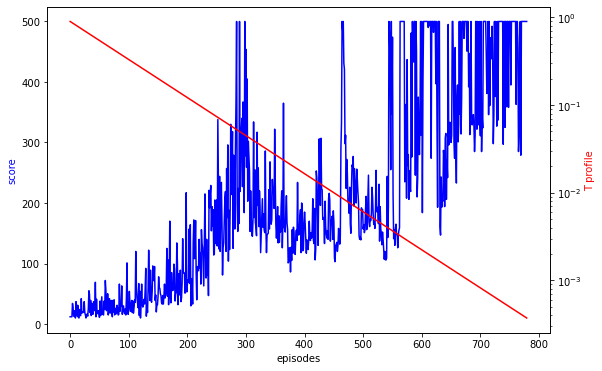
\includegraphics[width=0.45\textwidth]{img/vanilla2.png}} \quad
    \subfloat[$w_x=-0.2, e_x=4, w_\theta=-5, e_\theta=4$]{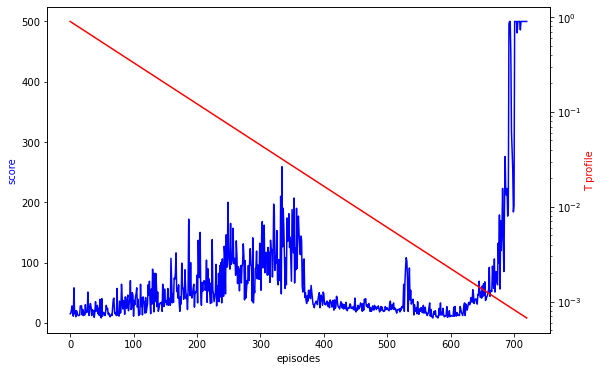
\includegraphics[width=0.45\textwidth]{img/mod_r_cv.png}} \\
    \subfloat[Wavy]{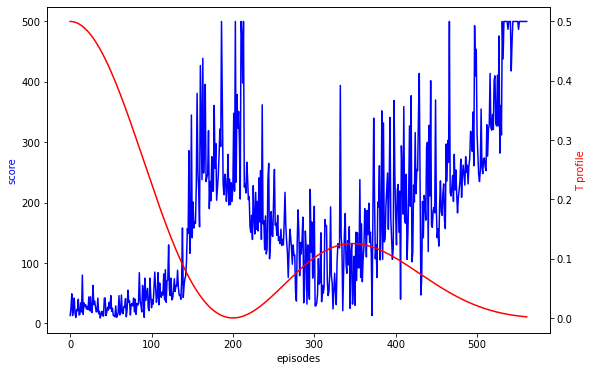
\includegraphics[width=0.45\textwidth]{img/wavy3.png}} \quad
    \subfloat[Best]{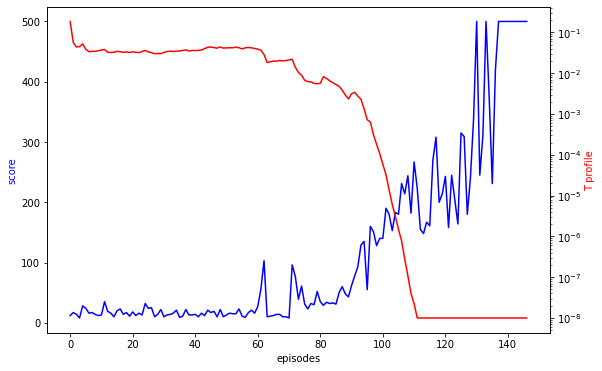
\includegraphics[width=0.45\textwidth]{img/best.png}}
    \caption{Behavior of the agent score and the softmax temperature during learning for four different cases.}
    \label{fig:scores}
  \end{figure}


\section{Cart-Pole with screen pixels}
  Dealing with the screen pixels is much harder than with the high level information provided to the agent so far and so to achieve good results relatively quickly one has to use more advanced methods.

  First of all the images are 3 channels rgb pictures of $600 \times 400$ pixels. The raw images are very heavy both to store in the replay memory and to process by the agent's policy net and also contain a lot of white space, so I proceeded to crop them (between 100 and 500 on the x axis and between 160 and 320 on the y axis), converted them to gray scale using only the blue channel (the one with the higher contrast), making the negative (as to have most of the pixels black, i.e. with value 0) and then downsampling the y axis, i.e. keeping only one row of pixel every 6 of them (fig \ref{fig:pixels} (a)).
  Also, since from a single picture there is no way of telling the velocity of the cart or of the pole, I provided the agent with four consecutive frames. So the resulting input for the policy net of the agent are tensors of shape $4 \times 27 \times 400$. To speed up the computations every time an image is saved in the replay memory, it is saved directly as a GPU tensor (and every sample contains 8 images: four for the 'state' and four for the 'next state'). For this reason I had to limit the replay memory capacity to 4000 samples.

  The policy network is now a convolutional network: I tried manually playing with its parameters and finally settled on three convolutional layers with [16,32,16] channels, kernel size of 4, stride of 2 and padding of 0, followed by a single hidden linear layer with 256 neurons and finally the output layer with 2 neurons. I also used the modified reward as previously taking $x$ and  $\theta$ from the original high level state of the environment, adding a -10 penalty to the reward when the pole falls. This time the optimization was performed using the RMSProp optimizer with learining rate $3\cdot10^{-4}$, a batch size of 32, $\gamma=0.97$ and updating the target net every 5 episodes. The exploration profile for the softmax temperature was the same 'interactive' one used for the best agent before with the only difference to set the temperature to 0 instead of $10^{-8}$ when the computed value is below $10^{-9}$.

  In general I observed that the agent managed to perform quite well, beating the game but not consistently, however as training proceeded the score got bad again. I think this is due to the limited size of the replay memory, so as the agent becomes good the memory contains mostly images in which the pole is almost vertical. This way when we perform gradient descent we overfit the region of the input space where the pole is vertical losing precision on the rest of the space. At this point when the agent finds itself in a critical situation (pole slightly tilted), its policy net no longer predicts the correct Q-values and so it takes the wrong decision, letting the pole fall.

  To counteract this effect I stopped learning when the agent successfully beats the game for 5 consecutive times (no more 10), but most importantly new samples are pushed to the replay memory only if the score of the previous episode was below 350. This method (which I called PINO (Push If Not Over)) worked very well (fig \ref{fig:pixels} (b), \url{code/pino2.mp4}), and after 314 episodes of training I tested the agent at zero temperature over 100 episodes obtaining 94 perfect scores with a best combo of 39 consecutive ones and an average score of 480, results which are comparable with the best agent using the high level information.

  Before reaching this result I tried other techniques such as pushing to the memory every $n$ frames or letting the agent choose a new action every $n$ frames, repeating the previous one when not deciding, as well as trying different preprocessing on the images; however none of them showed particularly promising results.

  \begin{figure}
    \centering
    \subfloat[Original and preprocessed image]{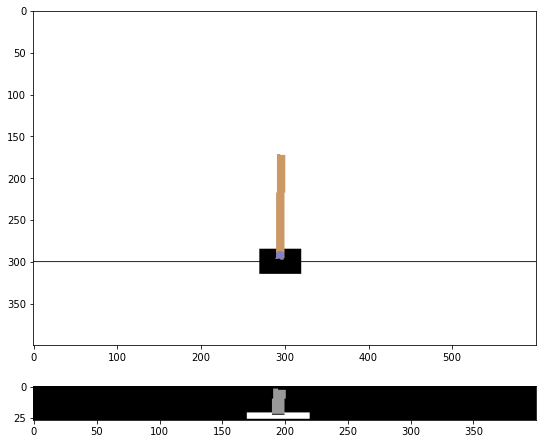
\includegraphics[width=0.4\textwidth]{img/preprocessing3.png}} \quad
    \subfloat[Trainng of the PINO agent]{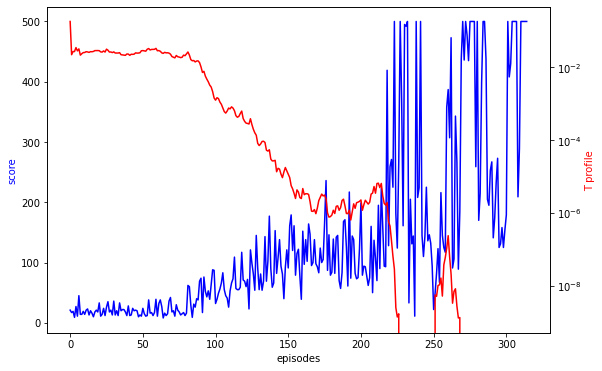
\includegraphics[width=0.5\textwidth]{img/pino2.png}}
    \caption{}
    \label{fig:pixels}
  \end{figure}



\section{Another gym environment: Acrobot}
  This environment consist of a double pendulum made of two bars of unitary length, where the joint between them is motorized: the agent has three available actions: namely applying to said joint a torque of -1, 0 or 1. The observation space consists of $[\cos(\theta_1), \sin(\theta_1), \cos(\theta_2), \sin(\theta_2), \dot{\theta_1}, \dot{\theta_2}]$ where $\theta_1$ is the angle of the first bar with respect to its rest position (pointing downward) and $\theta_2$ is $\pi$ minus the angle between the two bars.
  The height of the end point of the pendulum can be computed as $h = -(\cos(\theta_1) + \cos(\theta_1 + \theta_2) = \sin\theta_1\sin\theta_2 - \cos\theta_1 (1 + \cos\theta_2)$ and the goal is to achieve $h > 1$ before 500 steps (however I consider the game failed if the agent hasn't completed it in under 400 steps). In the vanilla version the agent receives a reward of -1 for every step until game termination and its score is minus the total number of steps.

  I tried training a simple net with two hidden layers with 128 neurons each, optimized with SGD with learning rate of 0.01, batch size of 128, $\gamma=0.97$  and updating the target net every 10 episodes and using an exponentially decaying profile for the softmax temperature.
  With this setup the agent was easily able to consistently (i.e. for 10 consecutive times) beat the game with less than 200 steps, but failed to beat it consistently in under 100 steps (fig \ref{fig:acrobot} (a)), so I tried modifying the reward from $r = -1$ to $r = -1 + w_h(h+2)^{e_h}$ and also adding a $P$ reward upon game termination. With $w_h=0.5, e_h=1, P=10$ the agent was able to consistently beat the game with less than 100 steps after 215 episodes of training (fig \ref{fig:acrobot} (b)). I tested it at zero temperature for 100 episodes obtaining an average score of -95.6.

  To conclude I tried to slightly complicate the environment by adding to the reward a penalty of -0.3 whenever the agent chooses to to use the motor , i.e. applying a +1 or -1 torque, with the idea of avoiding behaviors like the one in \url{code/acrobot_mod_r_bad.mp4} where the agent spins very fast without achieving much. To quantify how efficient the agent is in using the motor I introduce the quantity $\eta$ which is the fraction of actions which use the motor over an episode. I manually tweaked the reward parameters and then tested the final agent over 100 episodes, the results are in tab \ref{tab:acrobot} where we can see that by lowering $e_h$ below one the reward will steeply increase when the pendulum moves away from the resting position, but will then increase much slower when the pendulum is far from the equilibrium position, thus letting the agent optimize the efficiency of the motor usage. Also the increased efficiency doesn't affect drastically the agent's score.

  \begin{table}[H]
    \centering
    \begin{tabular}{ccc|ccc|c}
      \toprule
      motor penalty & $w_h$ & $e_h$ & training episodes & average score & $\eta$ & video example \\
      \midrule
      0 & 0.5 & 1 & 215 & -95.6 & 0.839 & \url{code/acrobot_mod_r.mp4} \\
      -0.3 & 0.5 & 1 & 830 & -93.93 & 0.796 & \url{code/acrobot_mc0.3.mp4} \\
      -0.3 & 0.5 & 0.5 & 1000 & -101.2 & 0.606 & \url{code/acrobot_mc0.3_eh0.5.mp4} \\
      -0.3 & 0.9 & 0.3 & 1000 & -133.6 & 0.477 & \url{code/acrobot_mc0.3_eh0.3.mp4}
    \end{tabular}
    \caption{Tests on the Acrobot trained with different rewards. In the last two rows the agent wasn't able to beat the game consistently in less than 100 steps, so learning stopped after 1000 episodes.}
    \label{tab:acrobot}
  \end{table}

  \begin{figure}
    \centering
    \subfloat[Vanilla]{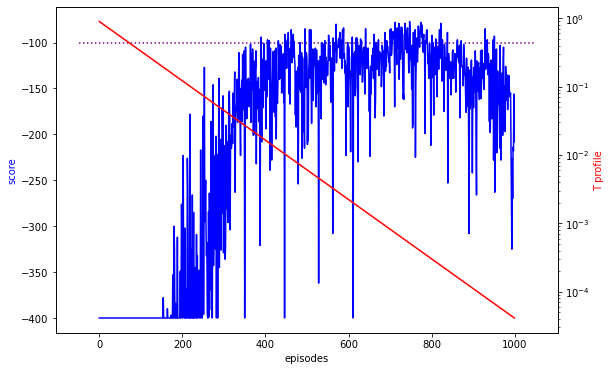
\includegraphics[width=0.3\textwidth]{img/acrobot_vanilla1.png}} \quad
    \subfloat[Modified reward]{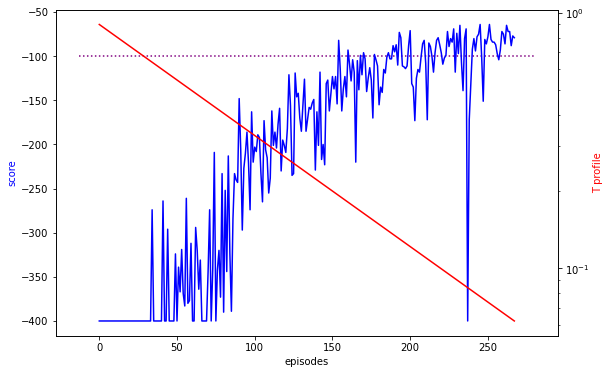
\includegraphics[width=0.3\textwidth]{img/acrobot_mod_r.png}} \quad
    \subfloat[Motor penalty]{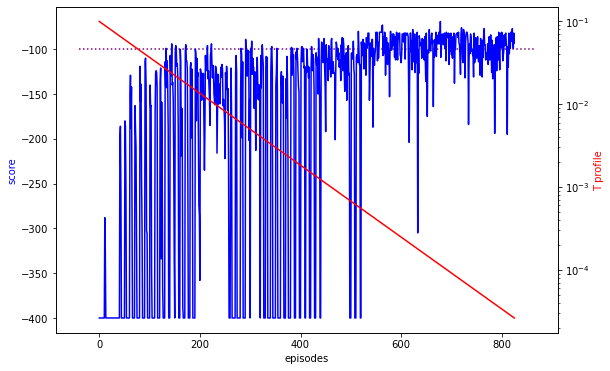
\includegraphics[width=0.3\textwidth]{img/acrobot_mod_r_motor0.3.png}}
    \caption{Score and temperature profile during training of the acrobot in the vanilla case and in the first tow rows of tab \ref{tab:acrobot}.}
    \label{fig:acrobot}
  \end{figure}









\end{document}
